\documentclass[11pt]{article}
\usepackage[utf8]{inputenc}
\usepackage{graphicx}
\usepackage{subfig}
\usepackage{enumerate}
\usepackage{fourier}
\usepackage[T1]{fontenc}
% \usepackage[letter,width=150mm, top=30mm, bottom=30mm]{geometry}
\usepackage[font={footnotesize}]{caption}
\usepackage[labelfont=bf]{caption}
\usepackage[english]{babel}
\usepackage{amsmath}
% \usepackage{fontspec}

\setlength{\parskip}{1em}
\graphicspath{{../figs/}}

\title{Practice Session 04: Energy Partitioning of Earthquake}
\author{Prithvi Thakur}
\date{Feb 27, 2019}

\begin{document}

\maketitle

% Problem 1
\section*{Stresses on the fault}
The effective normal stress ($\sigma_n$) increases linearly with depth ($z$), and the approxiamte gradient is $\sim 17\ MPa$.
\begin{equation}
\sigma_n = 17z\ MPa
\end{equation}

The static and dynamic shear strength depends on the assumed coefficient of friction ($\mu_s$ and $\mu_d$ respectively) and the effective normal stress as follows:
\begin{equation}
    \begin{aligned}
        \tau_s &= \mu_s \sigma_n \\
        \tau_d &= \mu_d \sigma_d \\
    \end{aligned}
\end{equation}

We use the values $0.6$ and $0.4$ for the static and dynamic coefficient of friction respectively.

Given a constant stress drop ($\Delta\sigma$) of $3\ MPa$, we can compute the shear stress before the earthquake ($\tau_0$) as:
\begin{equation}
    \tau_0 = \Delta\sigma + \tau_d
\end{equation}

\section*{Seismic Moment and Slip Calculation}
Given a moment magnitude ($M_w$) of $5$, we can calculate the seismic moment ($M_0$) as follows:
\begin{equation}
    M_0 = 10^{[\frac{3}{2}(10.7 + M_w) - 7]}
\end{equation}

The rupture dimension ($L$) is approximated as:
\begin{equation}
    L \sim \big(\frac{M_0}{\Delta\sigma}\big)^{\frac{1}{3}}
\end{equation}

The rupture area would therefore be $L^2$, and the final slip ($D_f$) is given by $\Delta\sigma L/G$, where $G$ is the shear modulus.

Based on these calculations and initial assumptions, we obtain the following values for a $M_w = 5$ earthquake:
\begin{equation}
    \begin{aligned}
        &M_w = 5 \\
        &\mu_s = 0.6 \\
        &\mu_d = 0.2 \\
        &M_0 = 3.55 \times 10^{16}\ Nm \\
        &L = 2279\ m \\
        &S = L^2 = 5.2 \times 10^6\ m^2 \\
        &D_f = 0.23\ m \\
        &D_c = 0.1\ m
    \end{aligned}
\end{equation}

where $D_c$ is the critical slip distance for the transition from static to dynamic friction.

\section*{Energy Calculations}
We use a simple linear slip-weakening model for calculations of energies. Fig. 1 shows the relation between stress and slip for the slip-weakening model. Based on this figure, the fracture energy ($E_g$) is estimated as the area $A'EC$ and the frictional/heat energy ($E_f$) is estimated as the area $OCBD$. The radiated energy ($E_r$) can be approximated as the area $ABC$. Therefore, using our variables defined above, we can estimate the energies as:
\begin{equation}
    \begin{aligned}
        E_g &= \frac{1}{2}\ D_c\ (\tau_s - \tau_d) S \\
        E_f &= D_f\ \tau_d S \\
        E_r &= \frac{1}{2}\ D_f\ (\tau_0 - \tau_d) S
    \end{aligned}
\end{equation}

Also, the total potential energy of the system is approximated as:
\begin{equation}
    \Delta W = \frac{1}{2}(\tau_0 + \tau_f) S D_f
\end{equation}

\begin{figure}[!htb]
    \centering
    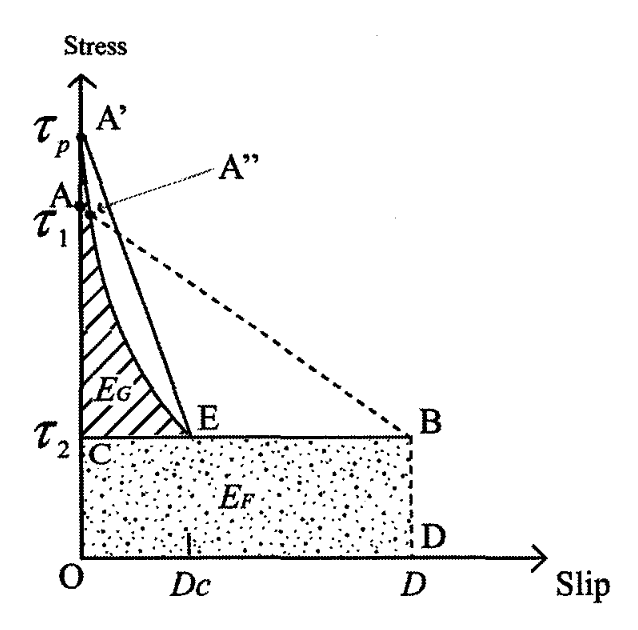
\includegraphics[scale=0.6]{eg.png}
    \caption{Ideal slip weakening model (Kanamori and Rivera, 2006)}
\end{figure}

The upper bound of radiated energy can also be estimated by subtracting the frictoin and fracture energy from the total potential energy, but this method gives negative values for radiated energies for the given $D_c$ and the moment magnitude. Therefore, we use the area of triangle to estimate the radiated energies for our calculations.

\section*{Results}
We show the energy partitioning at depth intervals of $1\ km$ from $3-15\ km$ and then their variation in depth. In our calculations, the radiated energy, as calculated from the area of the triangle, only depends on the stress drop and is constant with depth, but the relative contribution changes.

\begin{figure}[!htb]
    \centering
    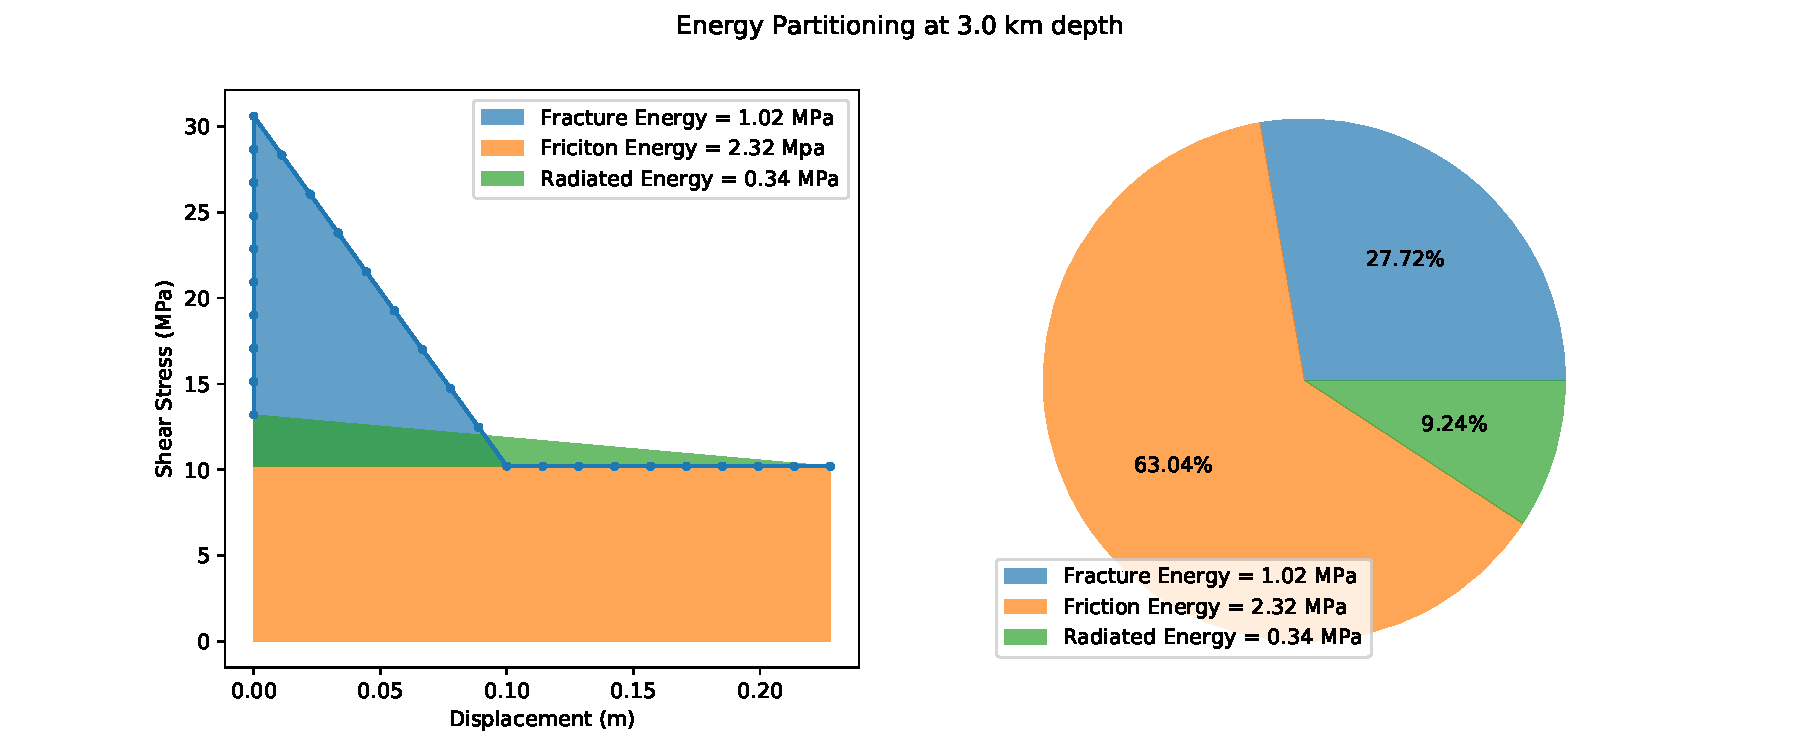
\includegraphics[scale=0.5]{depth3.pdf}\\
    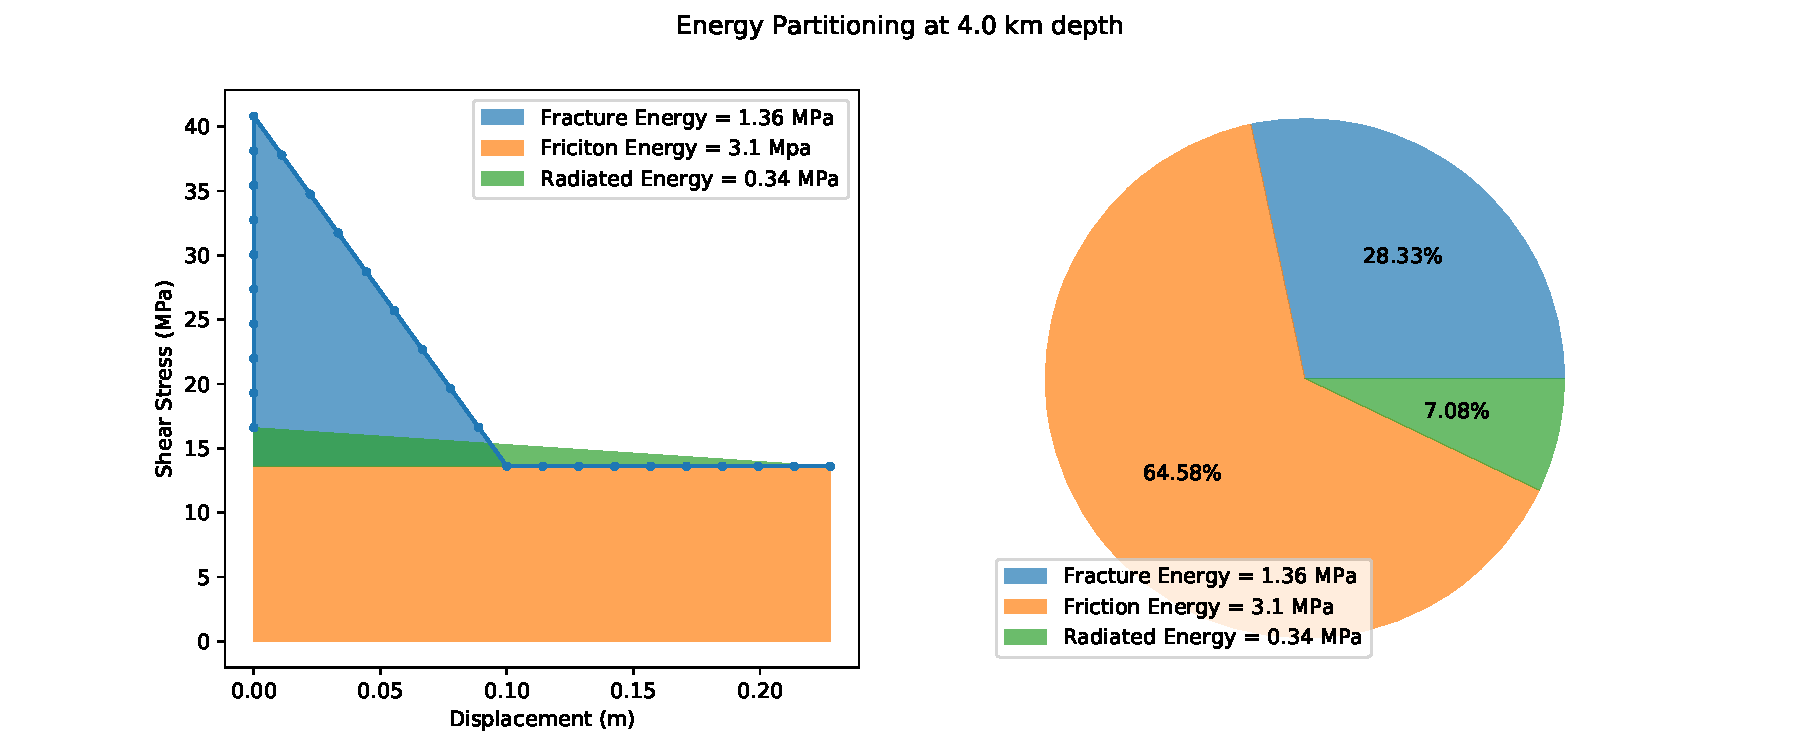
\includegraphics[scale=0.5]{depth4.pdf}\\
    % \caption{Ideal slip weakening model (Kanamori and Rivera, 2006)}
\end{figure}
\pagebreak
\begin{figure}[!htb]
    \centering
    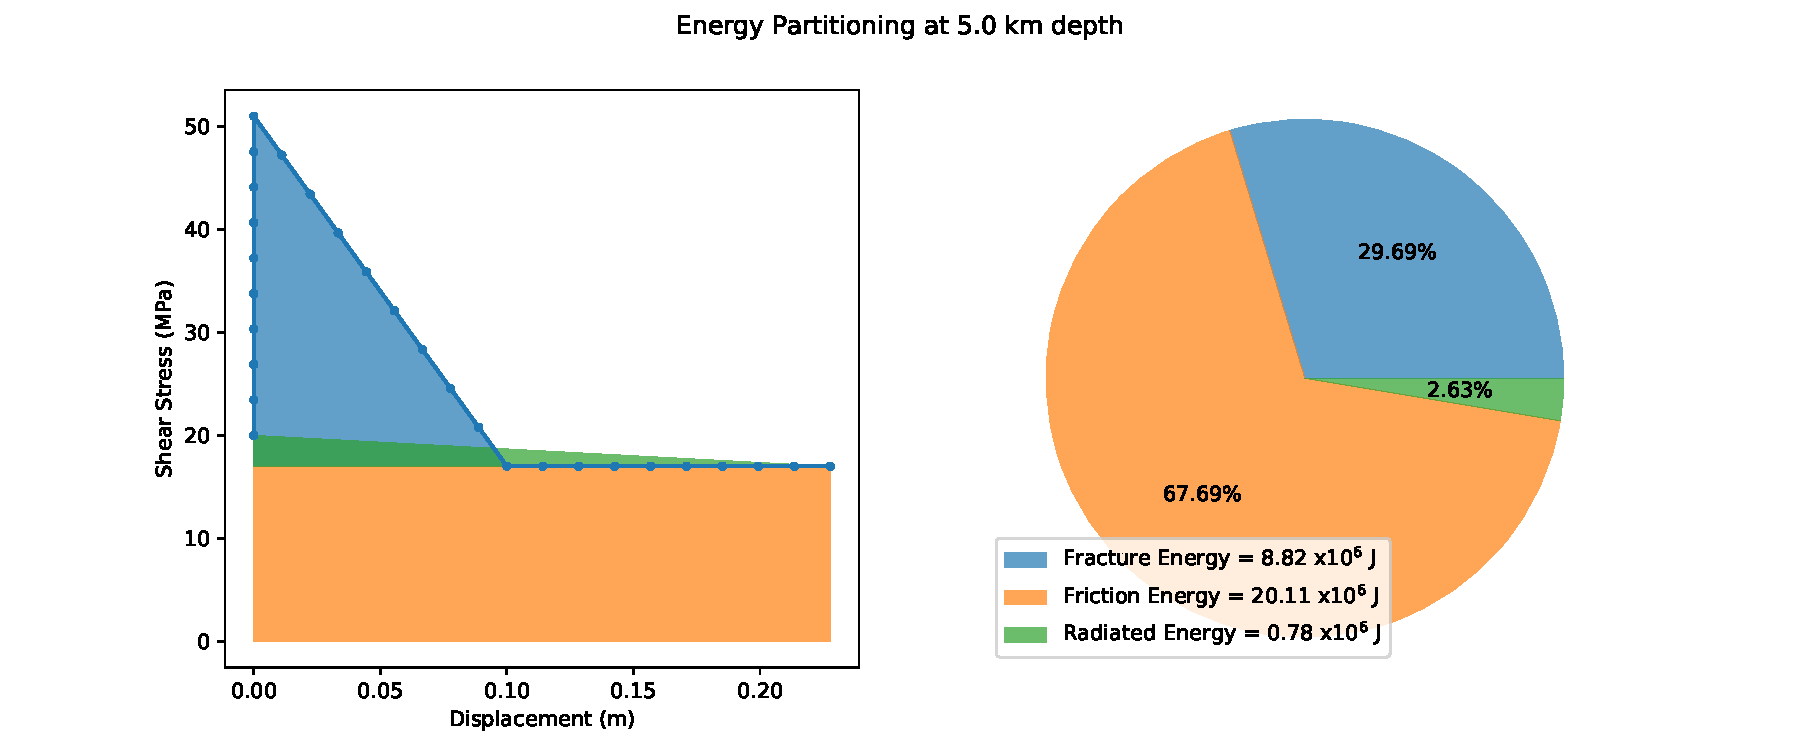
\includegraphics[scale=0.5]{depth5.pdf}\\
    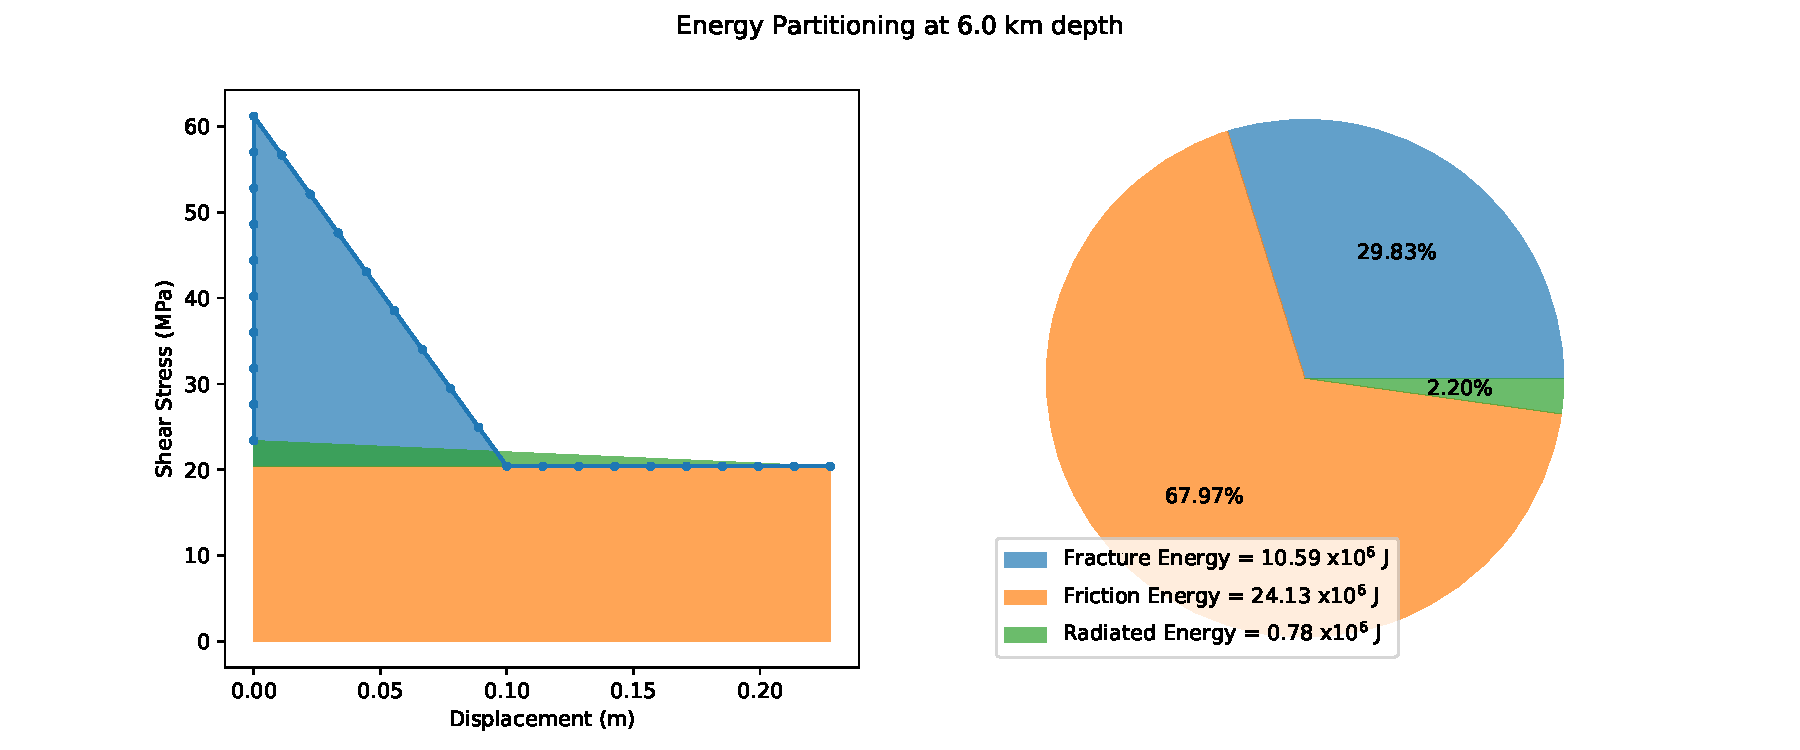
\includegraphics[scale=0.5]{depth6.pdf}\\
    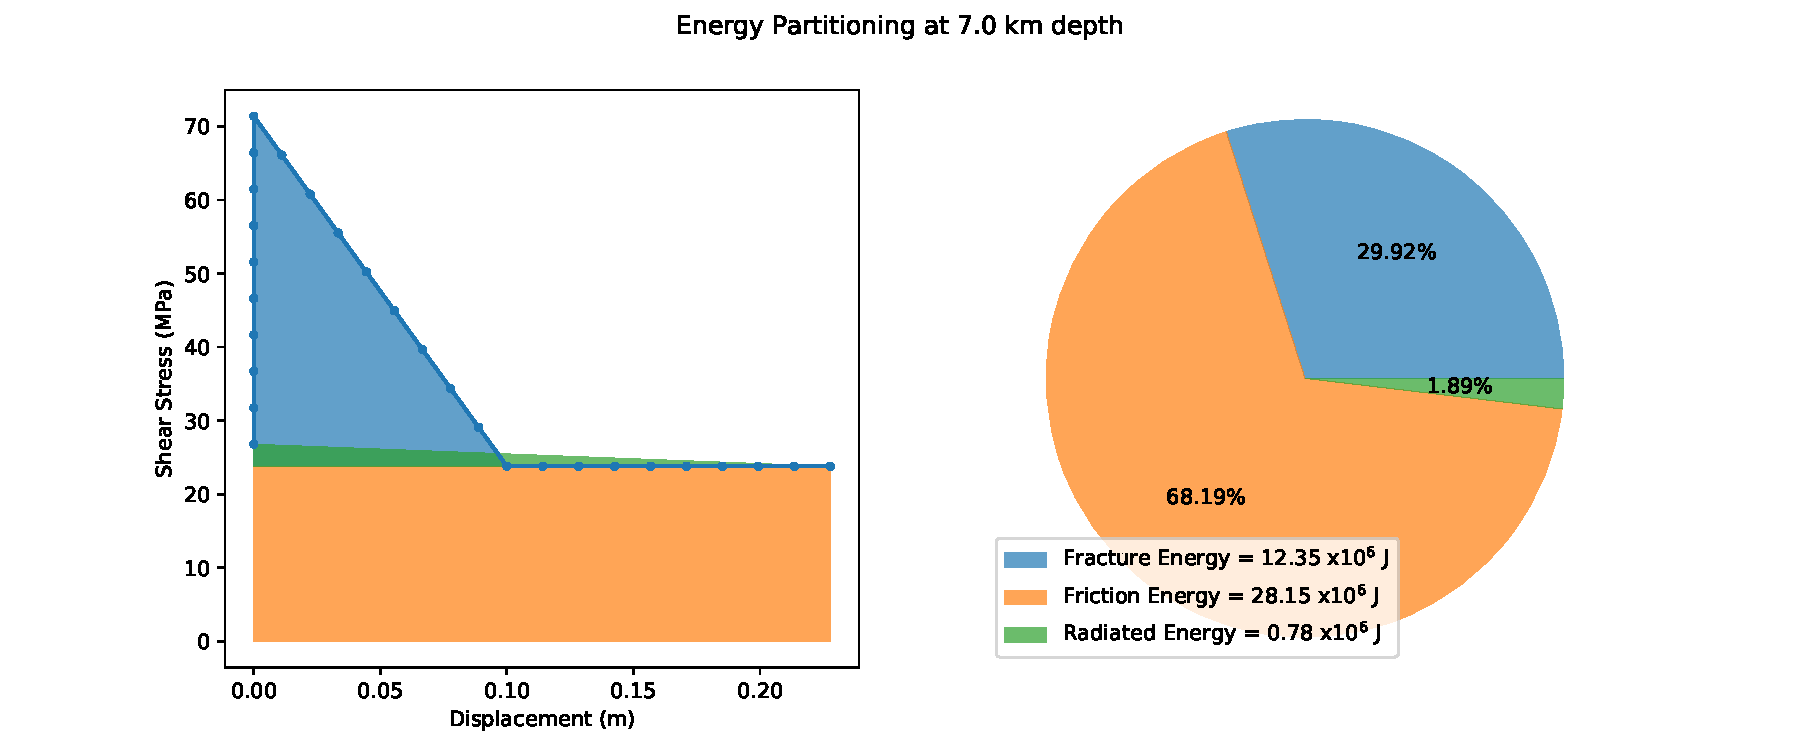
\includegraphics[scale=0.5]{depth7.pdf}\\
\end{figure}
\pagebreak
\begin{figure}[!htb]
    \centering
    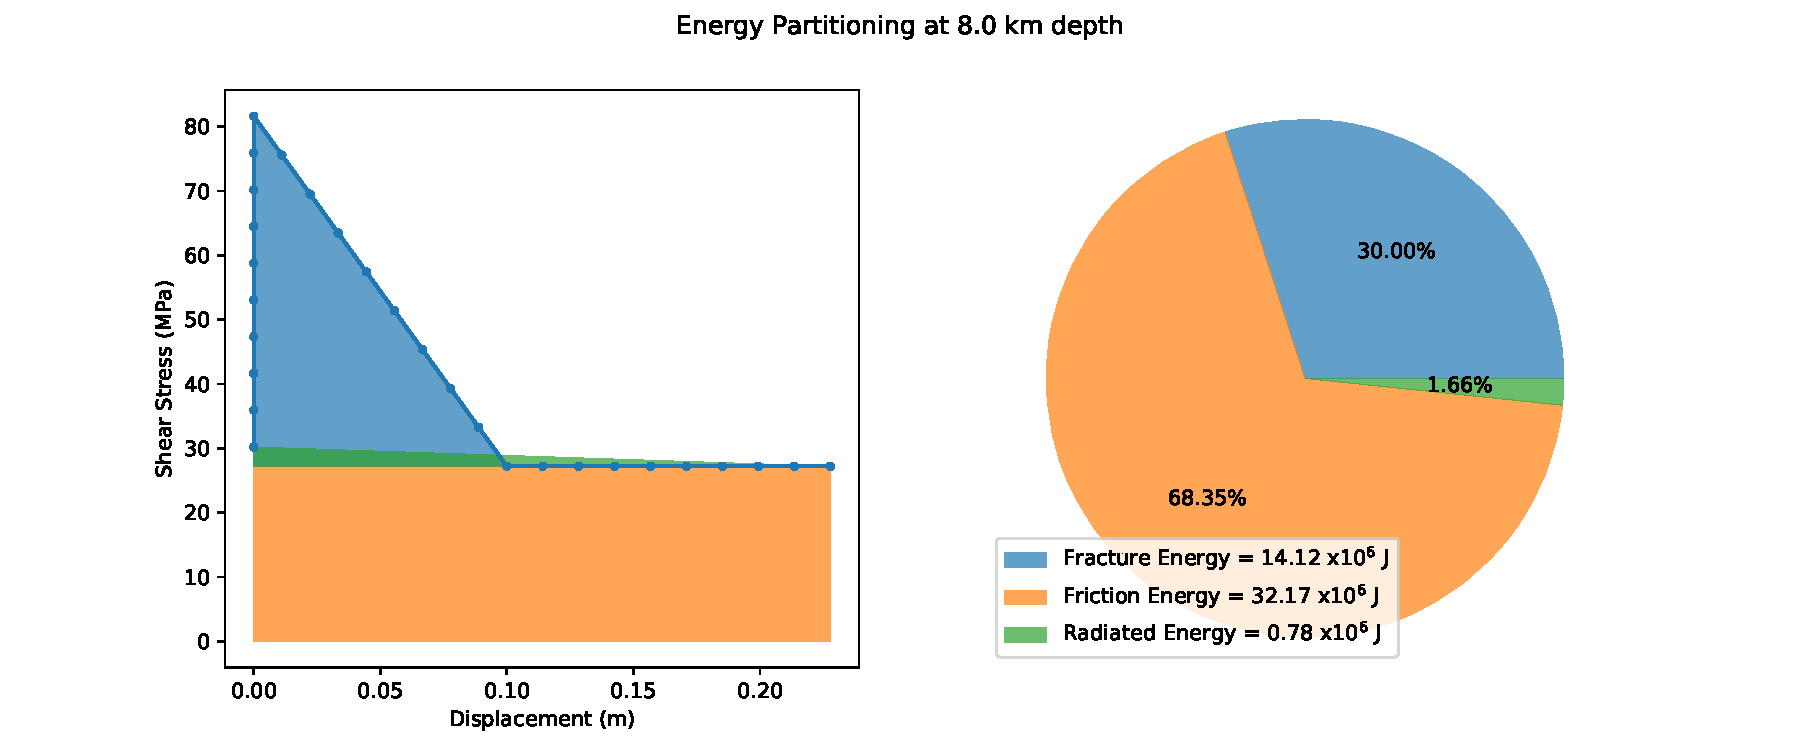
\includegraphics[scale=0.5]{depth8.pdf}\\
    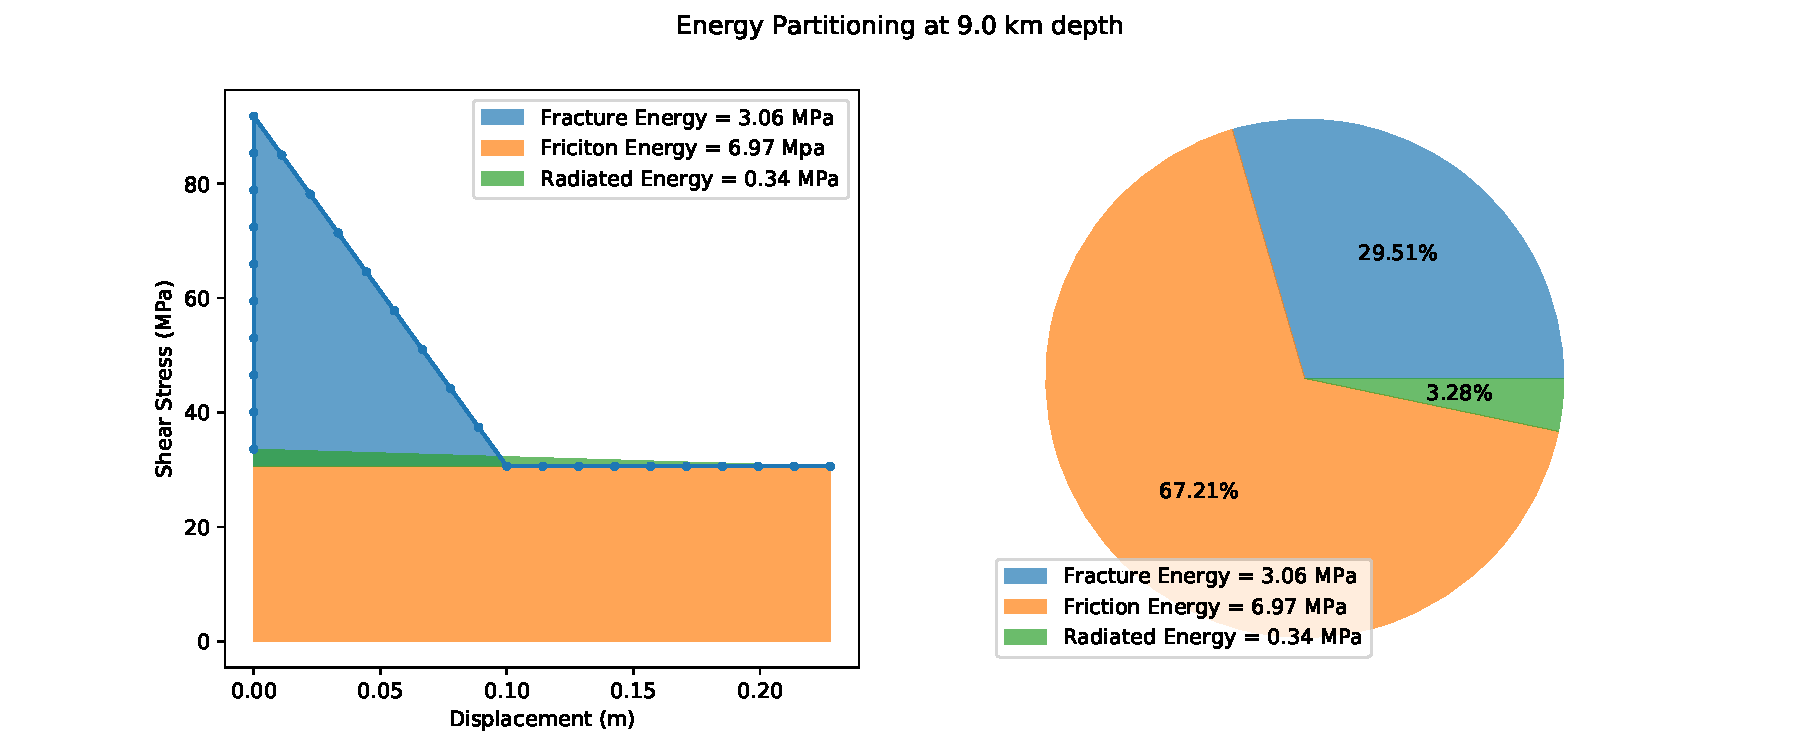
\includegraphics[scale=0.5]{depth9.pdf}\\
    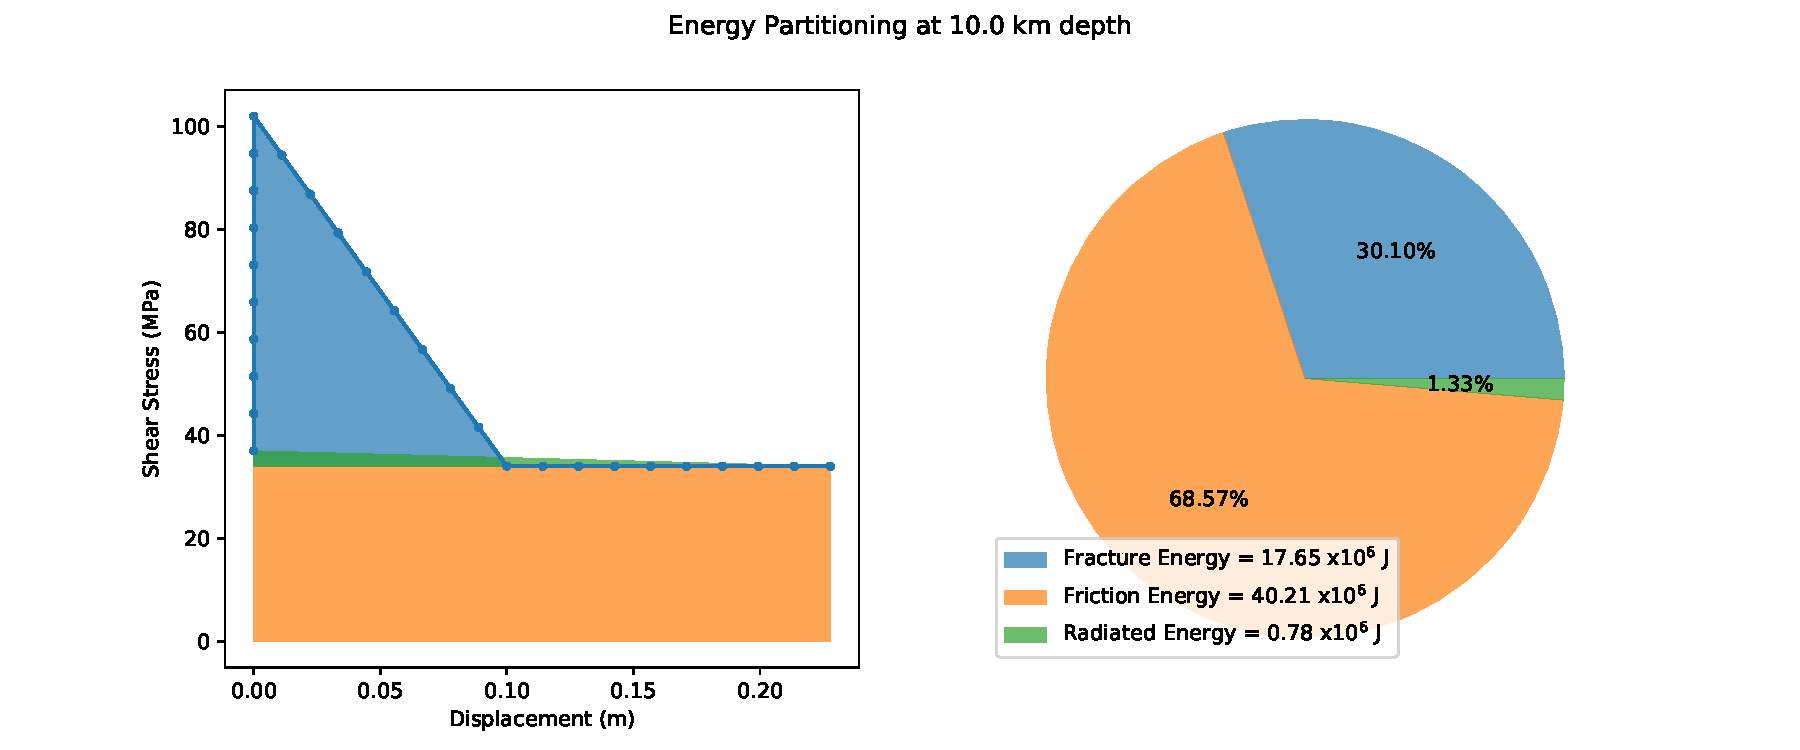
\includegraphics[scale=0.5]{depth10.pdf}\\
\end{figure}
\pagebreak
\begin{figure}[!htb]
    \centering
    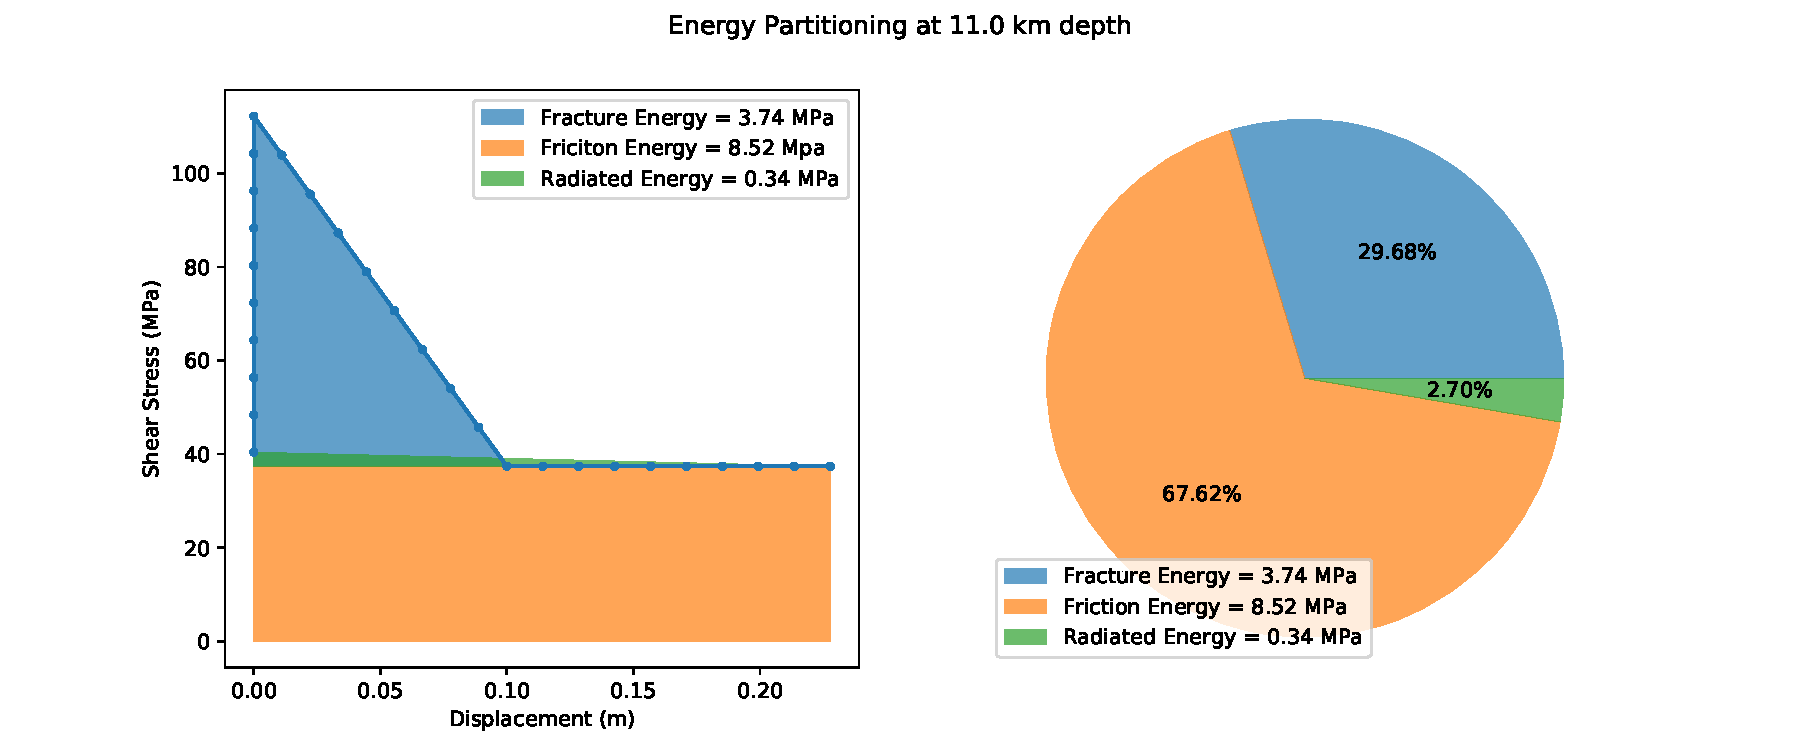
\includegraphics[scale=0.5]{depth11.pdf}\\
    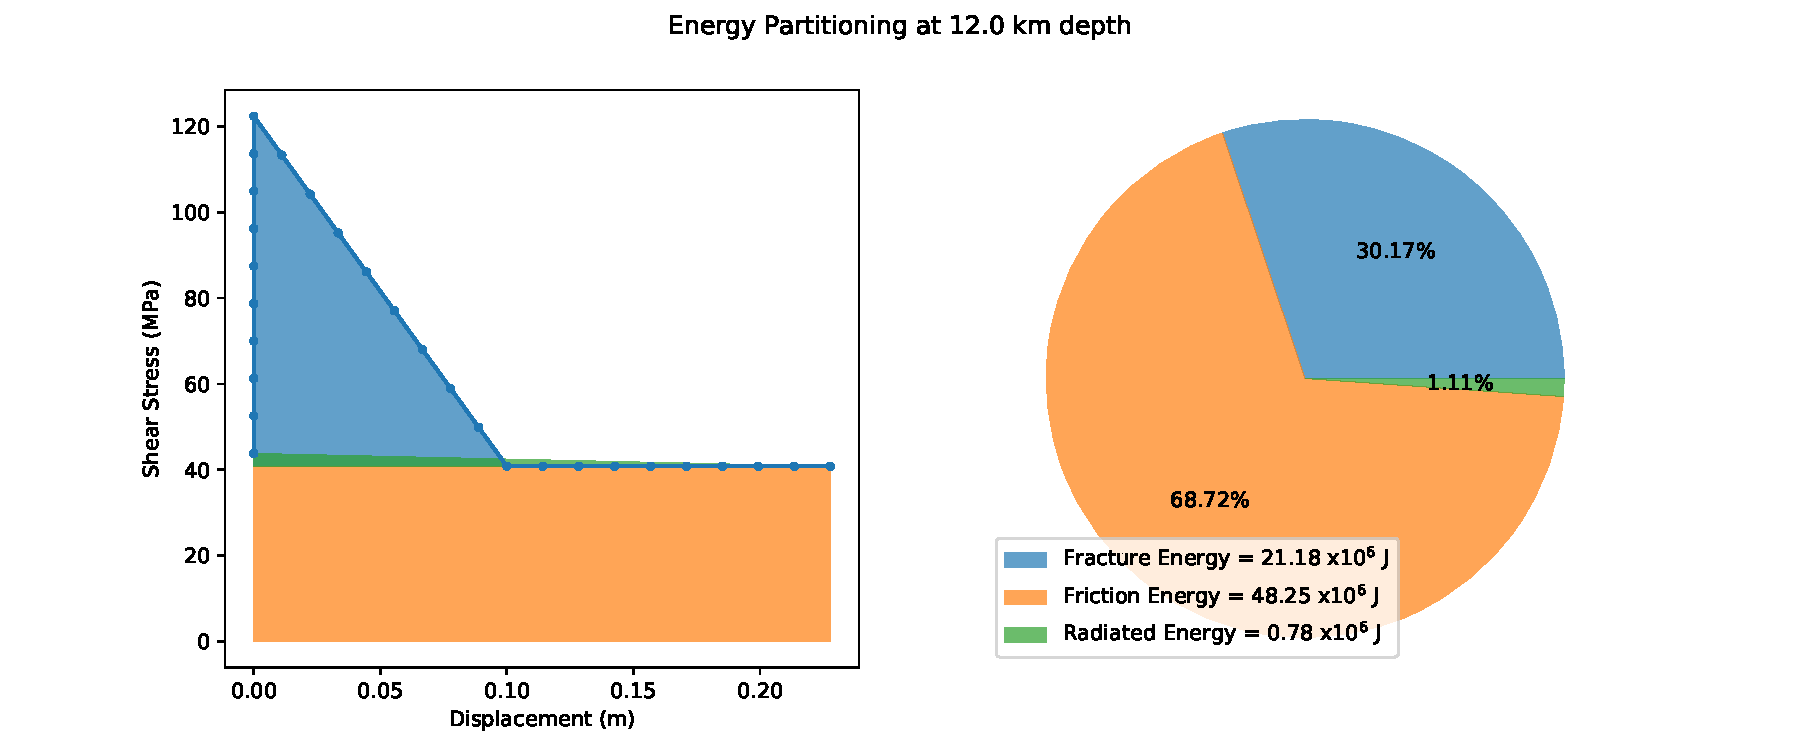
\includegraphics[scale=0.5]{depth12.pdf}\\
    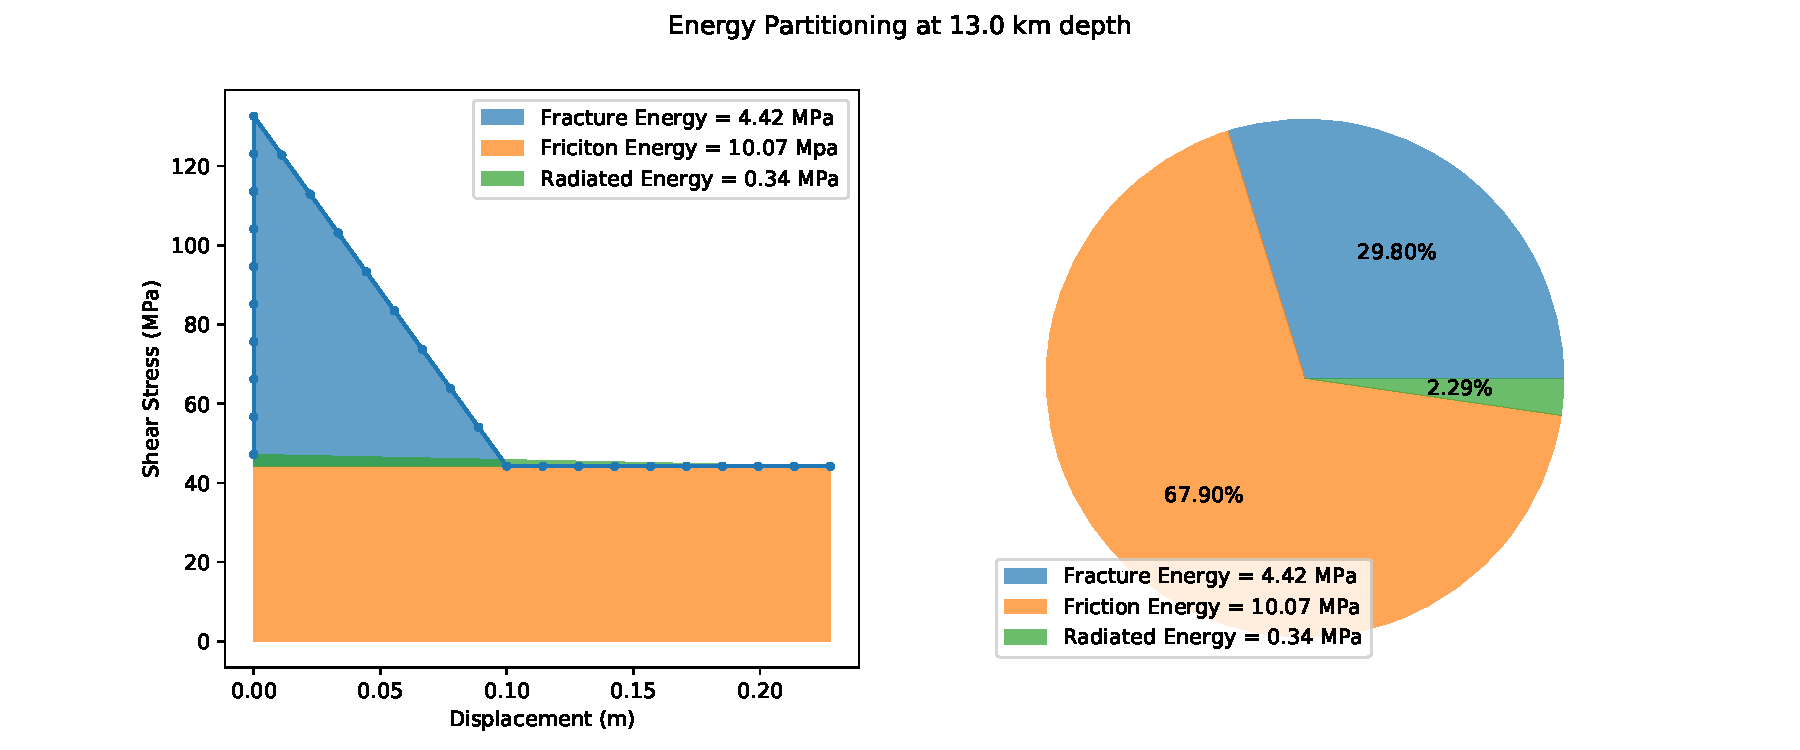
\includegraphics[scale=0.5]{depth13.pdf}\\
\end{figure}
\pagebreak
\begin{figure}[!htb]
    \centering
    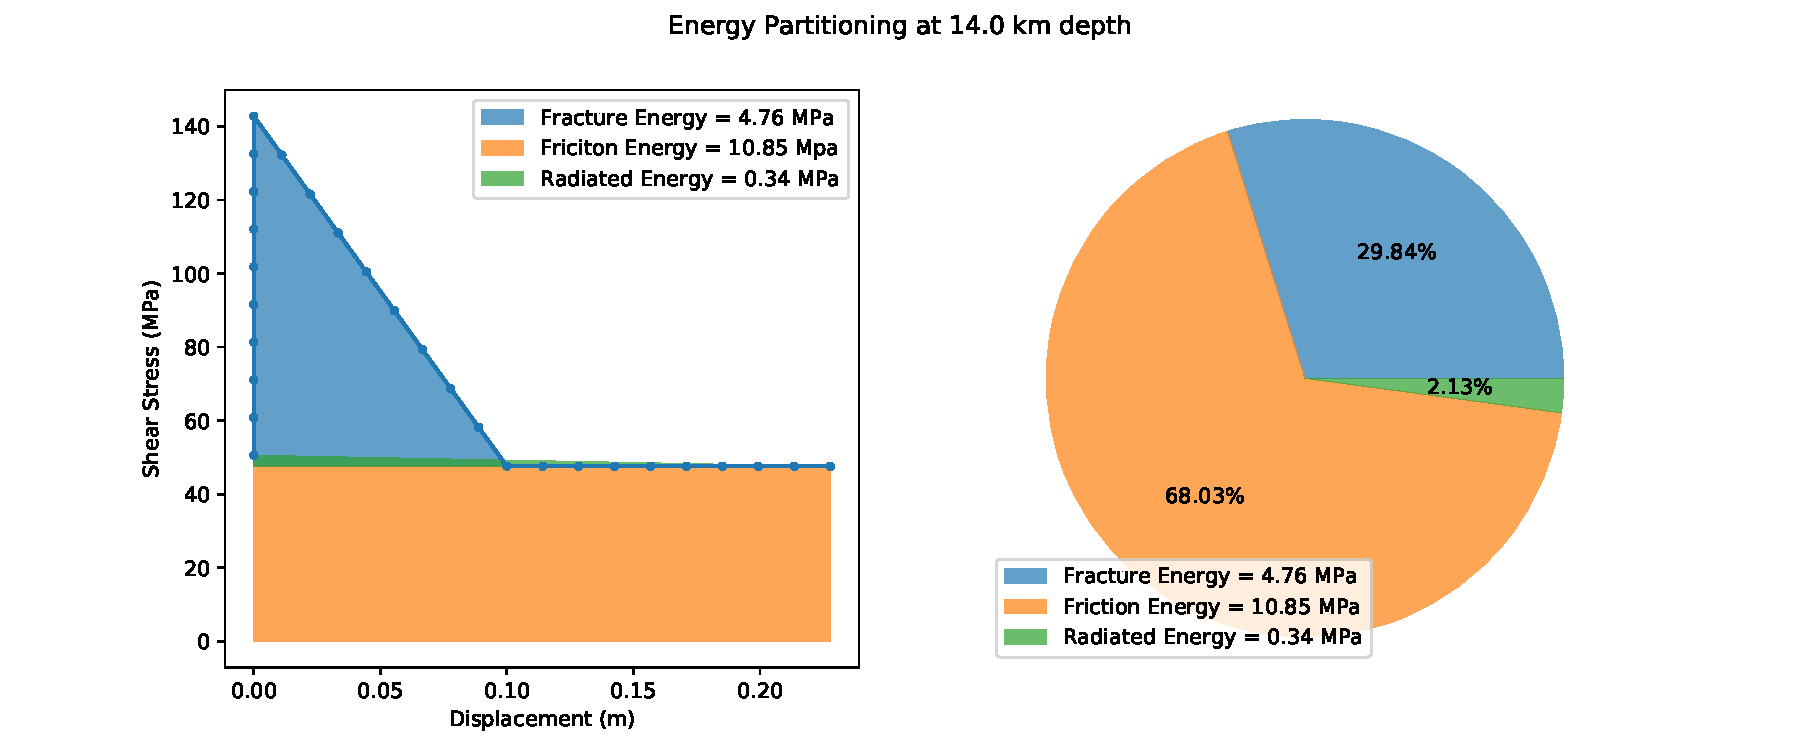
\includegraphics[scale=0.5]{depth14.pdf}\\
    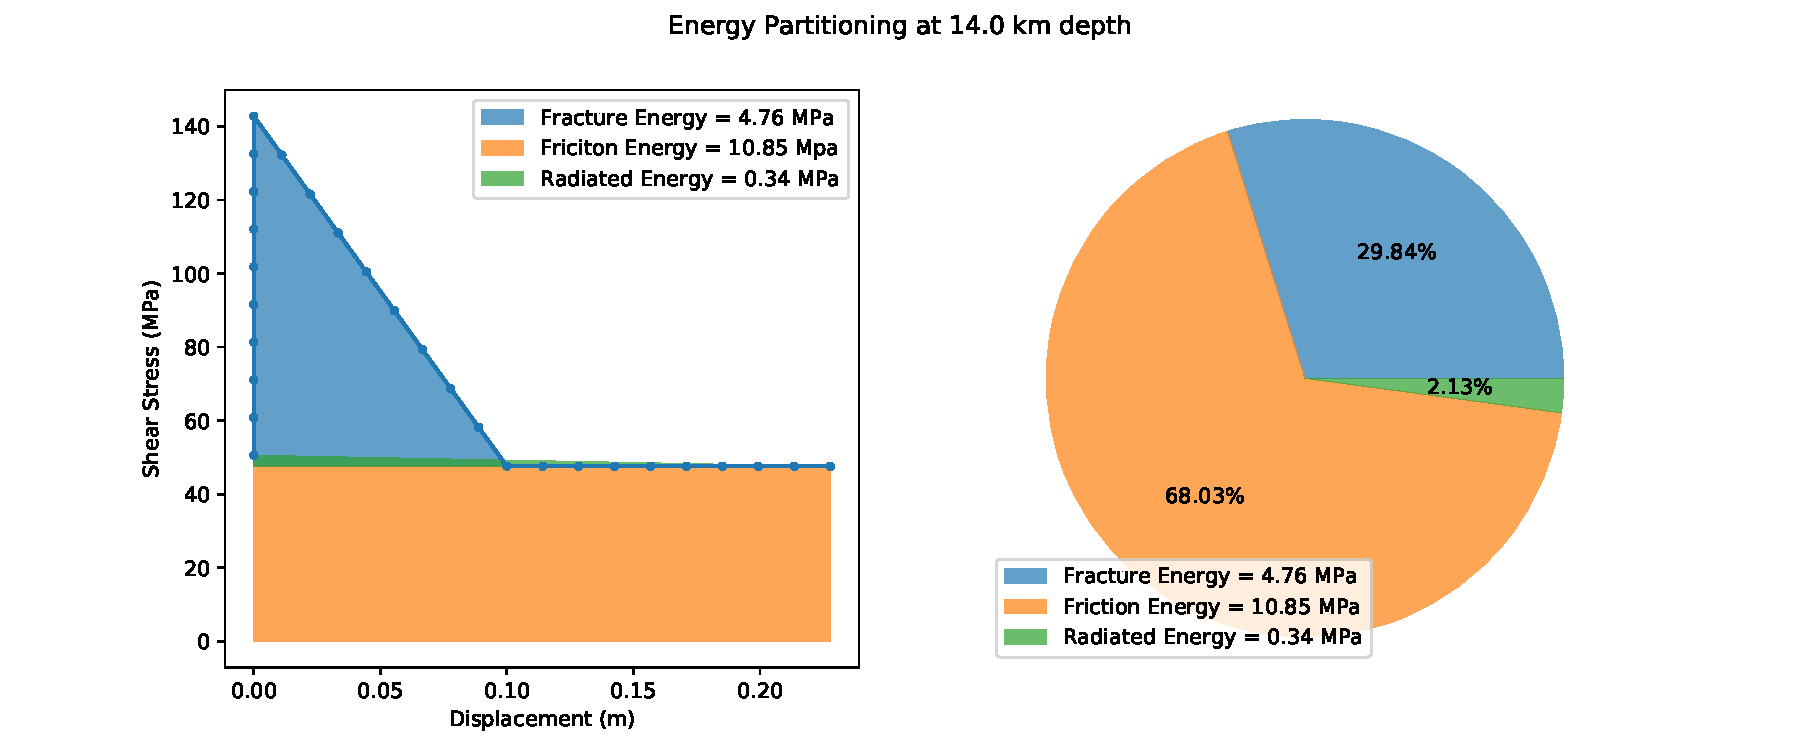
\includegraphics[scale=0.5]{depth14.pdf}\\
    \caption{Stress vs. Displacement and pie chart for energy partitioning. We use the area for calculation of radiated energies.}
\end{figure}
\clearpage

Next, we show the variation of the energies with depth. The Fig. 3 is plotted using the given values of input parameters $D_c$ and $M_0$. In Fig. 4, we reduce the $D_c$ in order to obtain positive values of radiated energies using the total potential energy. The radiated energy calculation from the area of the triangle does not change. Fig. 5 shows the energy partitioning for $M_w$ 7 earthquake.
\begin{figure}[!htb]
    \centering
    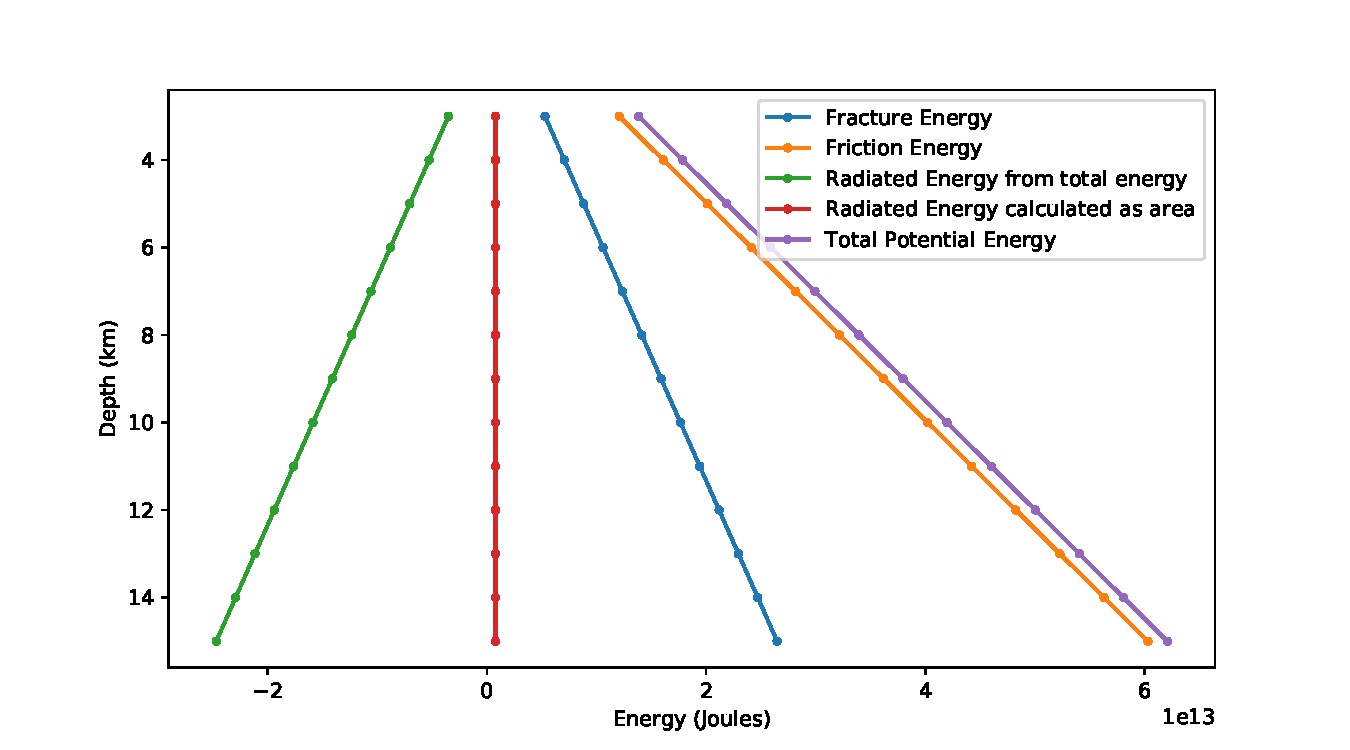
\includegraphics[scale=0.5]{energy_part_M5.pdf}\\
    \caption{Energy partitioning for $M_w$ 5 earthquake with $D_c = 0.1$ m.}
\end{figure}
\begin{figure}[!htb]
    \centering
    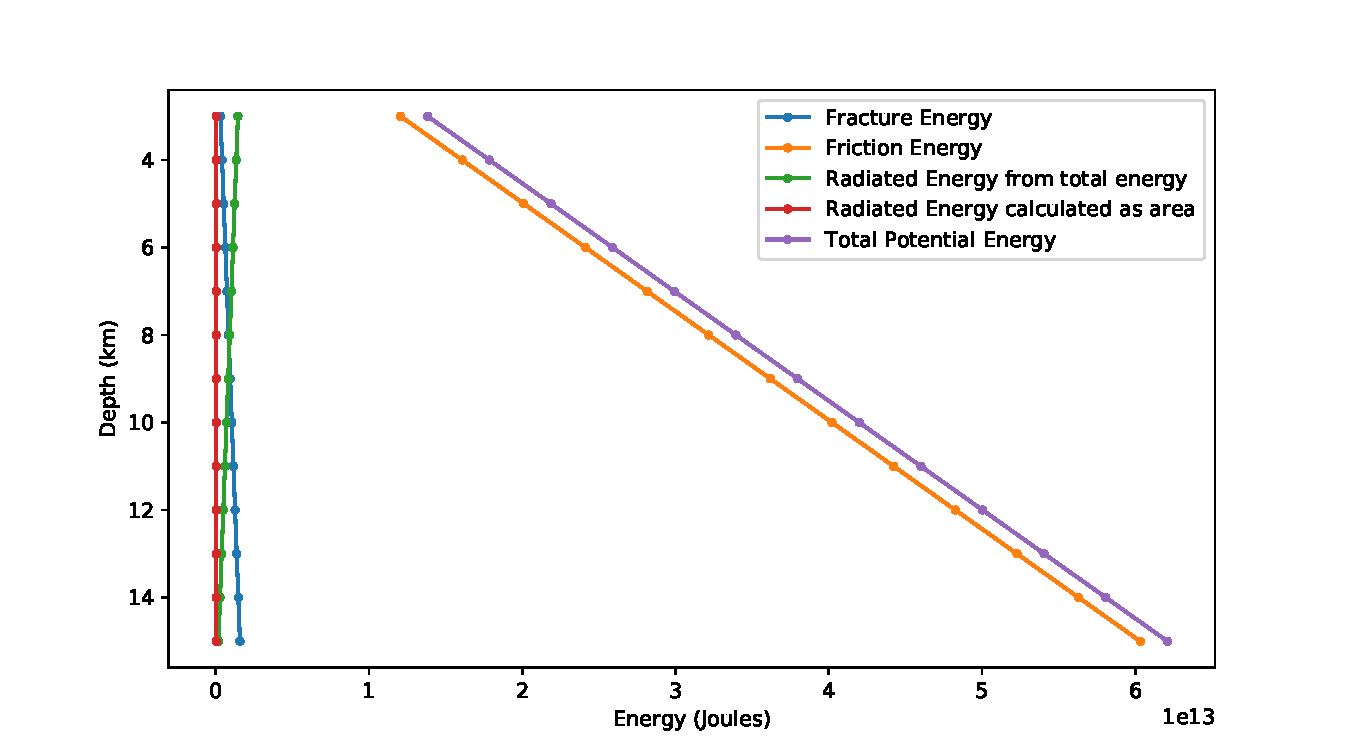
\includegraphics[scale=0.5]{energy_part_M5_2.pdf}\\
    \caption{Energy partitioning for $M_w$ 5 earthquake with $D_c = 0.006$ m.}
\end{figure}
\begin{figure}[!htb]
    \centering
    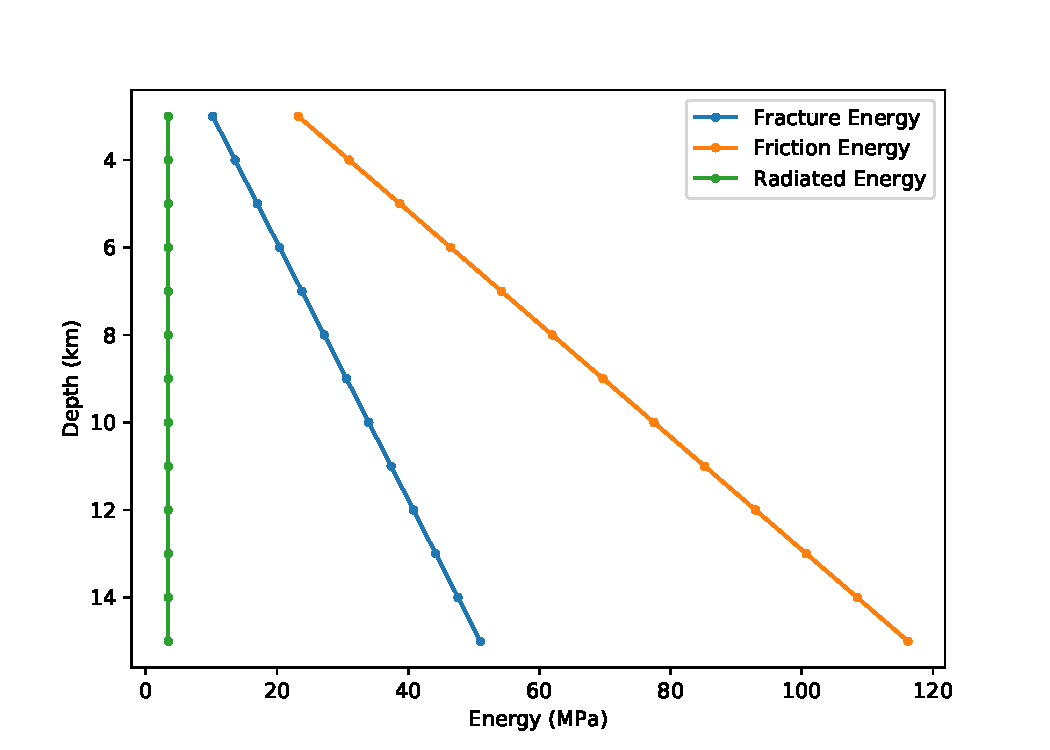
\includegraphics[scale=0.5]{energy_part_M7.pdf}\\
    \caption{Energy partitioning for $M_w$ 7 earthquake with $D_c = 1$ m.}
\end{figure}
\clearpage

\end{document}
